This section demonstrates how to control the Seven Segment Display through the
Dabble Android application using WiFi and display on the seven segment according
to the controls in the Android app.

\subsection{Connections}
\begin{enumerate}[label=\thesection.\arabic*.,ref=\thesection.\theenumi]
\numberwithin{equation}{enumi}
\numberwithin{figure}{enumi}
\numberwithin{table}{enumi}
\item \textbf{Note} :Components\ref{table:ble-components} and  Connections\ref{fig:vaman/uart/1},\ref{table:ble-connections} are similar to the bluetooth control seven segment display .
\item Now, execute the following code
\item Make sure that change your "ssid","password" in code 
\begin{lstlisting}
vaman-esp32/wifi/codes/src
\end{lstlisting}
\item Build ESP32 firmware.
\begin{lstlisting}
cd vaman-esp32/wifi/codes
pio run 
\end{lstlisting}
\item Flash ESP32 firmware (connect Arduino-UART).
\begin{lstlisting}
pio run -t upload
\end{lstlisting}
\item Now check that your mobile/tab is connected with ESP32.
\item Install the WiFi Dabble app.
\begin{lstlisting}
vaman-esp32/wifi/Wifi_dabble.apk
\end{lstlisting}

\item Open the Dabble application. Enter the Vaman-ESP32 IP address as shown 
in \ref{fig:dabble}.
\begin{figure}[!ht]
\centering
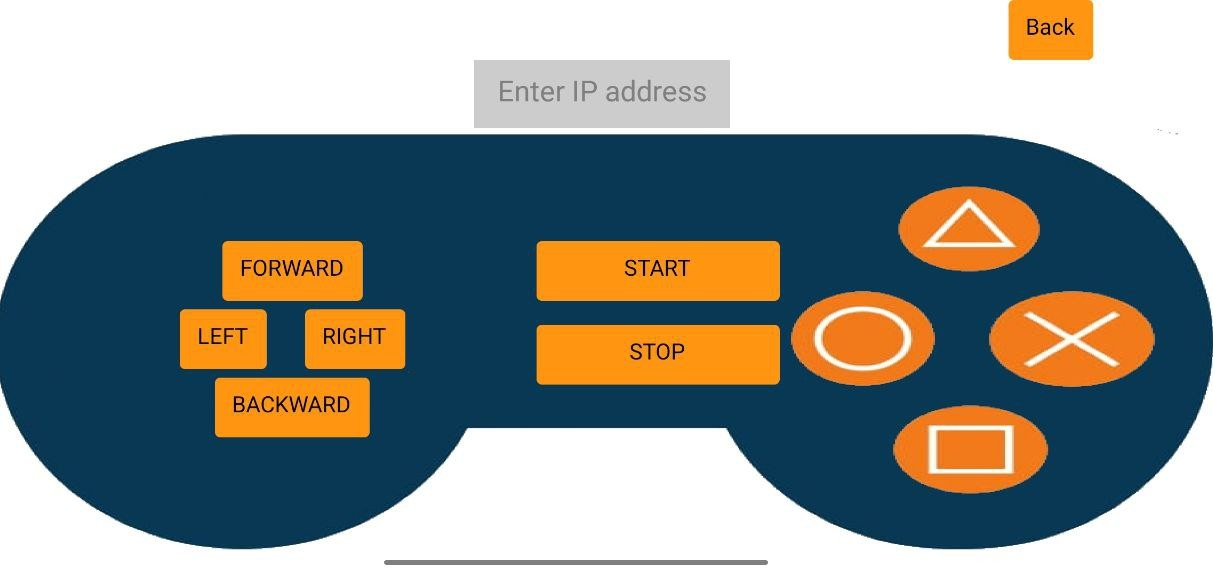
\includegraphics[width=0.6\columnwidth]{figs/wifi.jpg}
\caption{Wifi Dabble app}
\label{fig:dabble}
\end{figure}
\item Now you can observe the changes on seven-segment display for Start, Up, 
Down, Right and Left keys pressed on the Android application.
\end{enumerate}